\documentclass{article}
\usepackage[utf8]{inputenc}           % Use uft8 enconding to have a wide
                                      % number of symbols available
\usepackage[spanish]{babel}           % Configure the text language
                                      % to know where to put the hyphen in a 
                                      % line break
\usepackage{graphicx}                 % To include images
\usepackage{anysize}                  % Allows marginsize command
\usepackage{fancyhdr}                 % Configure the header and footer  
\usepackage{titlesec}                 % Changes the section titles properties
\usepackage{amsmath}                  % Active wide number of math symbols
\usepackage{amssymb}                  % Math symbols such as semijoin
\usepackage{longtable}                % Multiple-page table
\usepackage[export]{adjustbox}        % Allows to resize tables
\usepackage{enumitem}                 % Controls the item position 
\usepackage{listings}                 % Package for code fences
%\usepackage{xcolor}                   % Create colors
\usepackage[
  table,
  svgnames,
  dvipsnames
]{xcolor}                             % Colors for code fences and 
                                      %table (rowcolor)
\usepackage{textcomp}                 % Helps to display quotes symbols properly
\usepackage{array}                    % Align fix size columns in tables
\usepackage{multicol}
\usepackage{subcaption}

\decimalpoint%                        % Use dot instead of comma to write 
                                      % decimal numbers
\setlength{\parindent}{0in}           % No indentation at first paragraph

\renewcommand{\familydefault}{\sfdefault} % Changing font
\titleformat*{\section}{\large\bfseries}  % Change section size
\marginsize{1.5cm}{2cm}{1.2cm}{1.5cm}       % {left}{right}{above}{below}
\setlength{\headsep}{0.3in}               % Changing headsep length
                                          % headsep is the vertical length 
                                          % between header an text area
\lstset{upquote=true}                     % For display quotes and double 
                                          % quoutes in a better style

% Defining column content alignment for fix size columns
\newcolumntype{L}[1]{>{\raggedright\let\newline\\\arraybackslash\hspace{0pt}}m{#1}}
\newcolumntype{C}[1]{>{\centering\let\newline\\\arraybackslash\hspace{0pt}}m{#1}}
\newcolumntype{R}[1]{>{\raggedleft\let\newline\\\arraybackslash\hspace{0pt}}m{#1}}  

%%%%%%%%%%%%%%%%%%%%%%%%%%%%%%%%%%%%%%%%%%%%%%%%%%%%%%%%%%%%%%%%%%%%%%%%%%%%%%%
%%%%%%%%%%                        Code style                         %%%%%%%%%%
%%%%%%%%%%%%%%%%%%%%%%%%%%%%%%%%%%%%%%%%%%%%%%%%%%%%%%%%%%%%%%%%%%%%%%%%%%%%%%%

\definecolor{codegreen}{rgb}{0,0.6,0}
\definecolor{codegray}{rgb}{0.5,0.5,0.5}
\definecolor{codepurple}{rgb}{0.58,0,0.82}
\definecolor{backcolour}{rgb}{1,1,1}

\lstdefinestyle{mystyle}{
  backgroundcolor=\color{backcolour},   
  commentstyle=\color{codegreen},
  keywordstyle=\color{magenta},
  numberstyle=\tiny\color{codegray},
  stringstyle=\color{codepurple},
  %
  basicstyle=\ttfamily\footnotesize,
  captionpos=b,                    
  breakatwhitespace=false,         
  breaklines=true,                 
  keepspaces=true,                 
  showspaces=false,                
  showstringspaces=false,
  showtabs=false,                  
  %
  tabsize=2
  % Diplay number to the left
  % numbers=left,                    
  % numbersep=5pt,                  
}

\lstset{style=mystyle}


%%%%%%%%%%%%%%%%%%%%%%%%%%%%%%%%%%%%%%%%%%%%%%%%%%%%%%%%%%%%%%%%%%%%%%%%%%%%%%%
%%%%%%%%%%                        Header Style                       %%%%%%%%%%
%%%%%%%%%%%%%%%%%%%%%%%%%%%%%%%%%%%%%%%%%%%%%%%%%%%%%%%%%%%%%%%%%%%%%%%%%%%%%%%

\pagestyle{fancy}
\fancyhf{}
\renewcommand{\headrulewidth}{0pt}

% Right header
% The right header has 
%   the subject title,
%   subtitle and 
%   the university logo
\fancyhead[R]{
    \begin{tabular}{l}
        \materia \\ 
        \actividad%
    \end{tabular}
    \,% Adding space between titles and logo    
    \rule[-1.75\baselineskip]{0pt}{0pt}
    % Strut to ensure a 1/4 \baselineskip between image and header rule
    
\includegraphics[height=3\baselineskip,valign=c]{unam}
}

%%%%%%%%%%%%%%%%%%%%%%%%%%%%%%%%%%%%%%%%%%%%%%%%%%%%%%%%%%%%%%%%%%%%%%%%%%%%%%%
%%%%%%%%%%              Cover page generator command                 %%%%%%%%%%
%%%%%%%%%%%%%%%%%%%%%%%%%%%%%%%%%%%%%%%%%%%%%%%%%%%%%%%%%%%%%%%%%%%%%%%%%%%%%%%

\newcommand{\coverPage}{
\thispagestyle{empty}
  \begin{minipage}[t][5cm][t]{0.2\linewidth}
    
\includegraphics[width=2.5cm]{unam.jpg}

    \vspace{10cm}
    % The following space is mandatory to display correct layout

    
\includegraphics[width=2.5cm]{fiblack}
  \end{minipage}
  %
  \begin{minipage}[t]{0.7\linewidth}
    \vspace{-2.5cm}
    \LARGE{\textbf{\university}}\\
    \Large{\textbf{\faculty}} \\
  
    \large{\semestre}\\[2cm]
  
    \large{\textbf{\materia (\clave)}}\\
    \large{\textbf{Gpo: \grupo}}\\[5mm]
    \large{\textbf{Profesor:} \profesor}\\ [1.5cm]
    \begin{center}
        \LARGE{\textbf{\actividad}}\\
        \LARGE{\textbf{\titulo}}\\
    \end{center}
  
    \vspace{3.3cm}
  
    \large{\textbf{Alumno:} \alumno} \\[1.5cm]
    %\large{
    %  \begin{itemize}[ noitemsep, align=left ]
    %    \item [\textbf{Alumno(s):}] 
    %      \begin{flushright}
    %        \alumno
    %      \end{flushright}
    %  \end{itemize}
    %} \vspace{1.5cm}
  
    \begin{flushright}
        \fechaEntrega%
    \end{flushright}
  \end{minipage}

\newpage
}

\begin{document}

%%%%%%%%%%%%%%%%%%%%%%%%%%%%%%%%%%%%%%%%%%%%%%%%%%%%%%%%%%%%%%%%%%%%%%%%%%%%%%%
%%%%%%%%%%                Variables definition                       %%%%%%%%%%
%%%%%%%%%%%%%%%%%%%%%%%%%%%%%%%%%%%%%%%%%%%%%%%%%%%%%%%%%%%%%%%%%%%%%%%%%%%%%%%

\newcommand{\university}{Universidad Nacional Autónoma de México}
\newcommand{\faculty}{Facultad de Ingeniería}
\newcommand{\semestre}{2021-1}
\newcommand{\materia}{BDA}
\newcommand{\clave}{2929}
\newcommand{\grupo}{1}
\newcommand{\profesor}{Ing. Rodriguez Campos \textsc{Jorge Alberto}}

\newcommand{\alumno}{Francisco Pablo \textsc{Rodrigo}}
\newcommand{\actividad}{Tema 04 \\ Ejercicio práctico 03}
\newcommand{\titulo}{Administración de las estructuras de memoria}

\newcommand{\fechaEntrega}{01 de enero de 2021}

\newcommand{\codedir}{tema04-ej-prac-03-codigo}
\graphicspath{{assets/}{tema04-ej-prac-03.assets/}}

\coverPage%


%%%%%%%%%%%%%%%%%%%%%%%%%%%%%%%%%%%%%%%%%%%%%%%%%%%%%%%%%%%%%%%%%%%%%%%%%%%%%%%
%%%%%%%%%%                        Contents                           %%%%%%%%%%
%%%%%%%%%%%%%%%%%%%%%%%%%%%%%%%%%%%%%%%%%%%%%%%%%%%%%%%%%%%%%%%%%%%%%%%%%%%%%%%

\section*{Objetivo}

Prácticar y explorar el uso de las vistas del diccionario de datos asociadas 
con el uso, administración y monitoreo de las áreas de memoria que componen
a la PGA

\section*{C1. Código y consulta de la tabla \texttt{t01\_redo\_log\_buffer}}

\lstinputlisting[language=SQL]{\codedir/s-01-redo-log-buffer.sql}

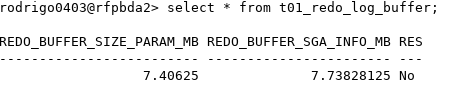
\includegraphics[width=0.5\linewidth]{c1}

\section*{C2. Código y consulta de la tabla \texttt{t03\_pga\_stats}}

\lstinputlisting[language=SQL]{\codedir/s-03-pga-stats.sql}

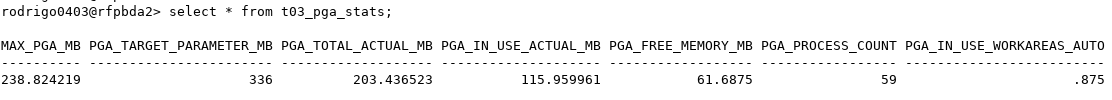
\includegraphics[width=\linewidth]{c2}

\section*{C3. Código y consulta de la tabla \texttt{t04\_pga\_process}}

\lstinputlisting[language=SQL]{\codedir/s-04-pga-process.sql}

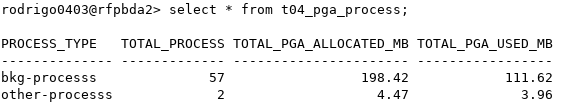
\includegraphics[width=0.6\linewidth]{c3}

\section*{C4. Evidencia configuración sentencias \texttt{insert} en JMeter y 
Log Viewer}

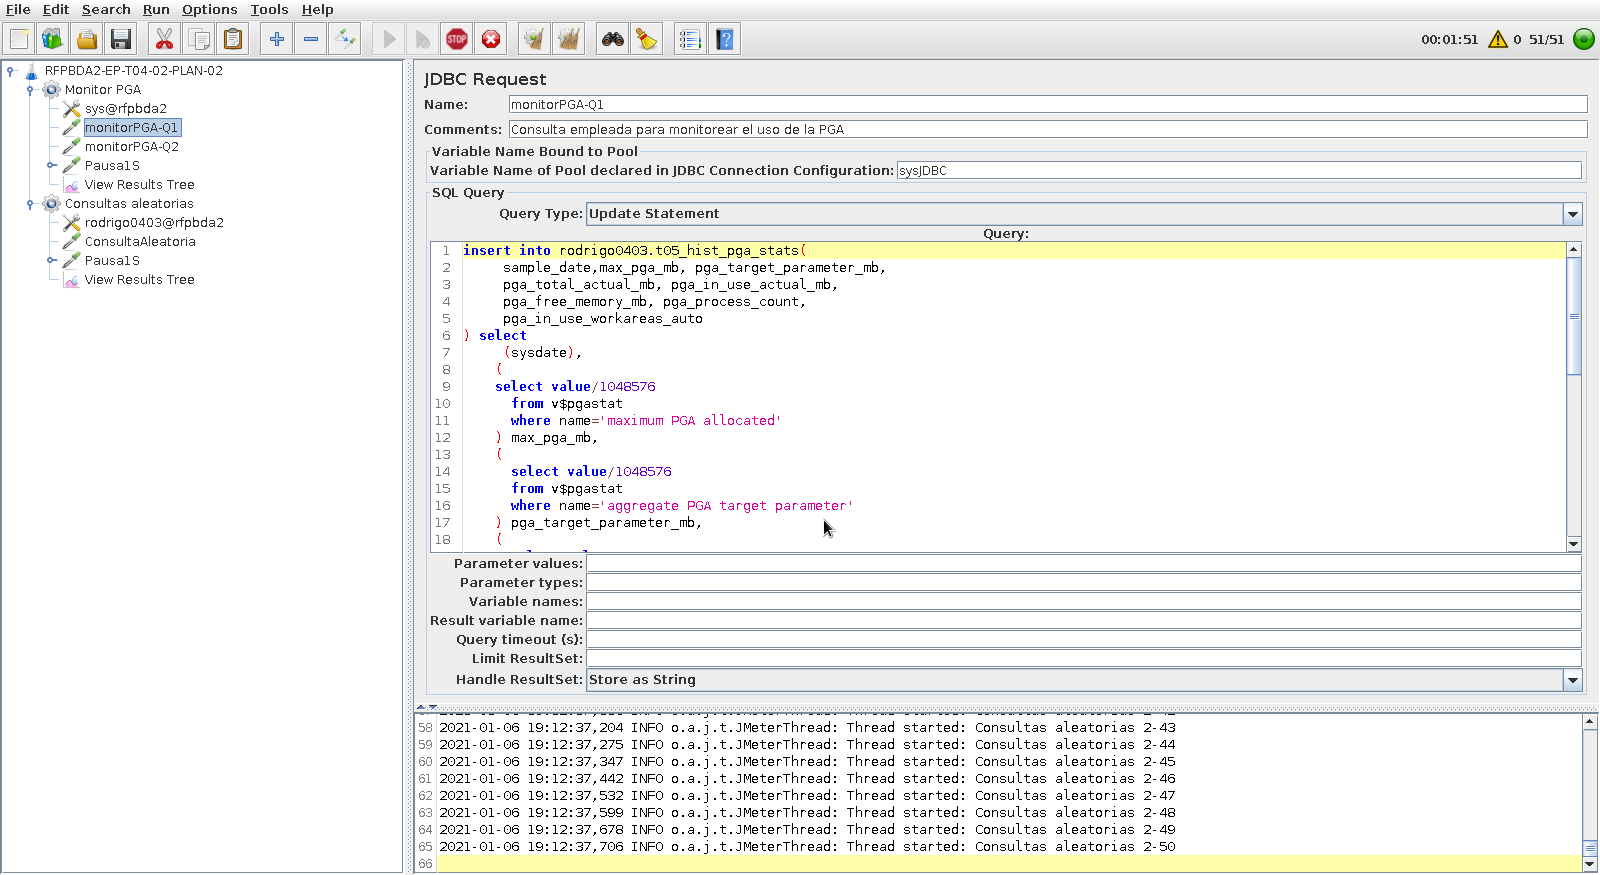
\includegraphics[width=\linewidth]{c4}

\section*{C5. Gráficas y explicación de monitoreo.}

\subsection*{Uso de la PGA}

\begin{figure}[ht!]
  \begin{subfigure}{0.5\textwidth}
    \centering  
    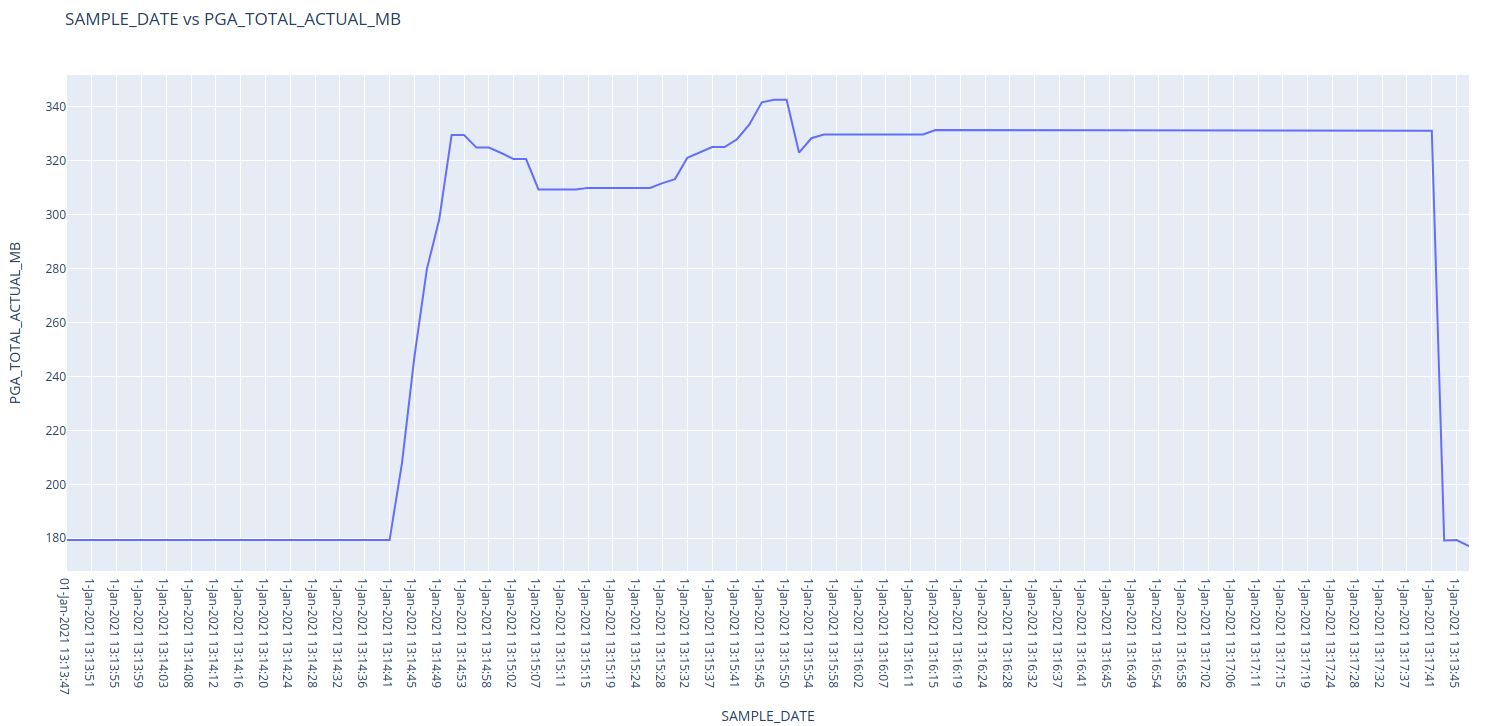
\includegraphics[width=0.9\linewidth]{t05-grafica01}
    \caption{}
  \end{subfigure} 
  \begin{subfigure}{0.5\textwidth}
    \centering  
    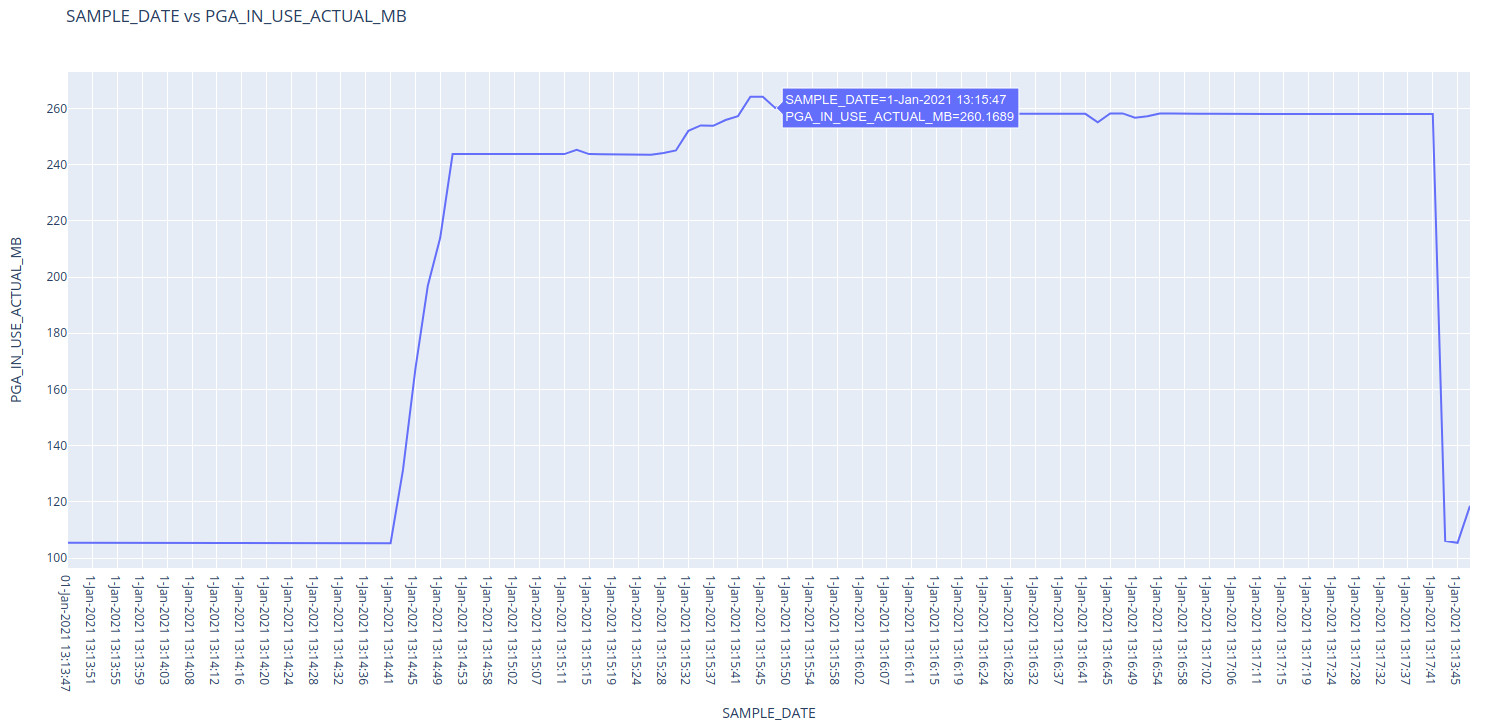
\includegraphics[width=0.9\linewidth]{t05-grafica02}
    \caption{}
  \end{subfigure} 
  \newline
  \\[3mm]
  \begin{subfigure}{0.5\textwidth}
    \centering  
    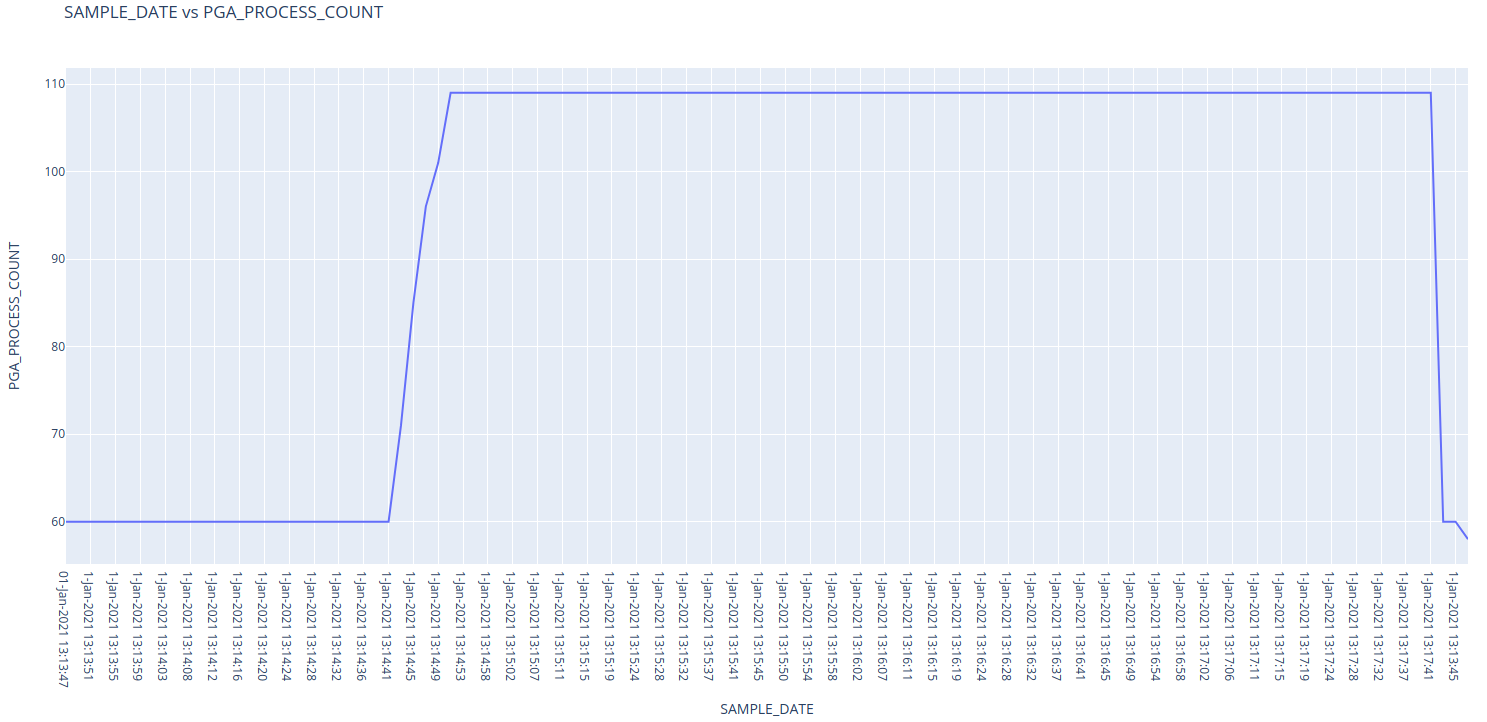
\includegraphics[width=0.9\linewidth]{t05-grafica03}
    \caption{}
  \end{subfigure} 
\end{figure}

En la primera y segunda gráfica (a y b) se muestra el uso de memoria por parte
de la PGA. Se puede observar que en el primer minuto (antes de que se empiecen a
crear los hilos del lado de jmeter) permance en un nivel relativamente bajo. Sin
embargo a la hora de empezar a realizar la consulta de los datos se empieza a
requerir de más memoria por lo que la PGA tiene que empezar a crecer. Un
comportamiento esperado era que el valor de la PGA se mantuviera relativamente 
constante, lo anterior se debe a que utilizamos una sentencia preparada y por lo
tanto no fue necesario compilar y almacenar la sentencia cada vez que se
ejecutará. 

Por otra parte, en el conteo de procesos, se observar se tiene que crear
procesos extra después del primer minuto para poder atender a los 100 hilos de
Jmeter. Una vez que estos terminaron su ejecución se observa que se eliminan
esos procesos y solo permanecen los que están por "default".

\subsection*{Uso de la PGA respecto a v\$process}

\begin{figure}[ht!]
  \begin{subfigure}{0.5\textwidth}
    \centering  
    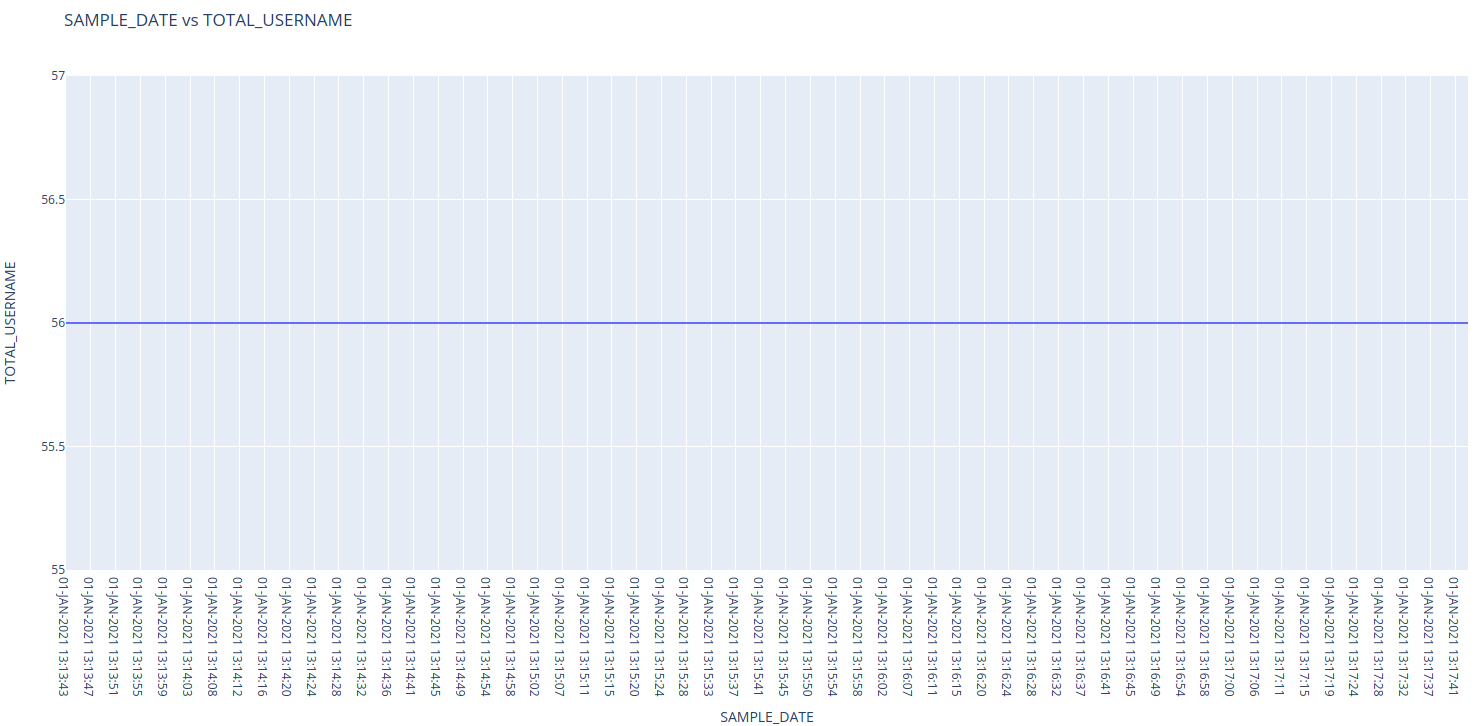
\includegraphics[width=0.9\linewidth]{t06-grafica01-bkg}
    \caption{Usando \texttt{bkg-processs}}
  \end{subfigure} 
  \begin{subfigure}{0.5\textwidth}
    \centering  
    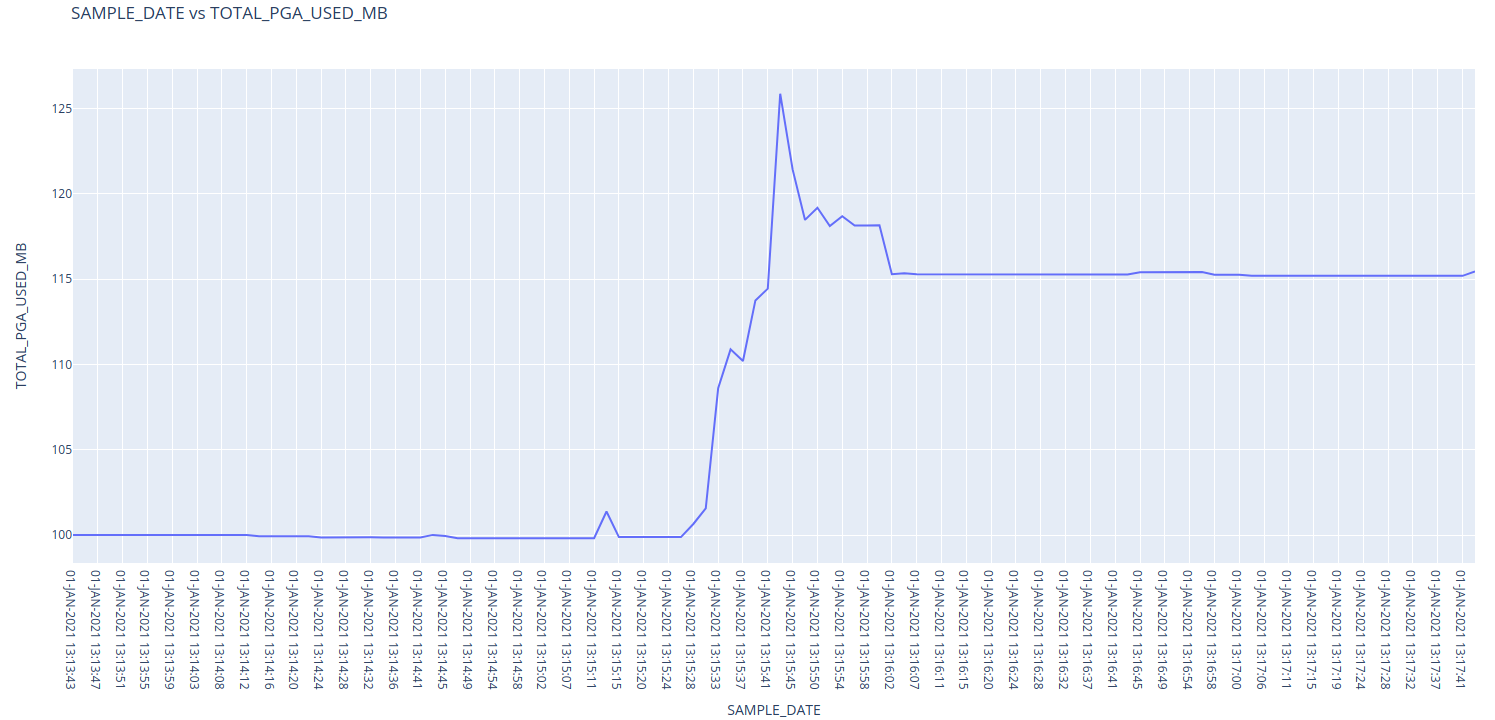
\includegraphics[width=0.9\linewidth]{t06-grafica02-bkg}
    \caption{Usando \texttt{bkg-processs}}
  \end{subfigure} 
  \newline 
  \begin{subfigure}{0.5\textwidth}
    \centering  
    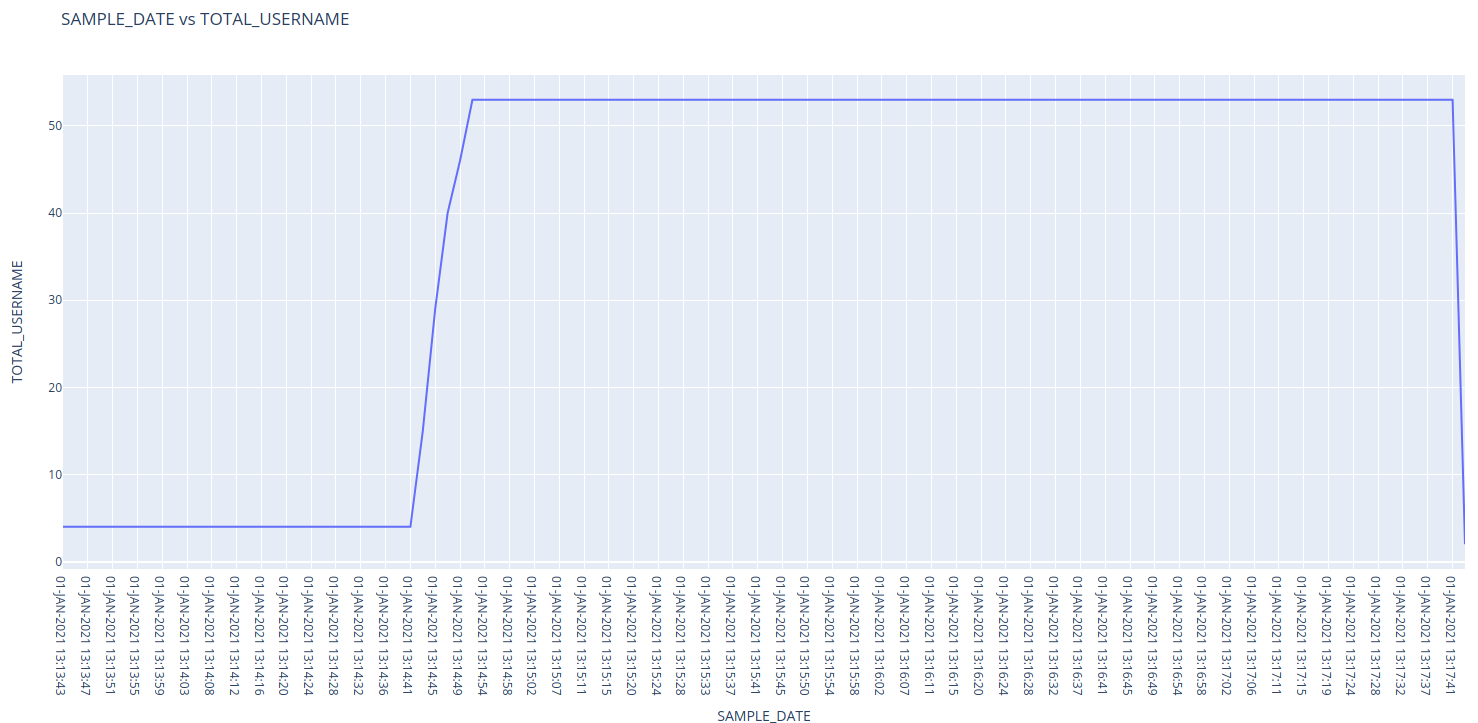
\includegraphics[width=0.9\linewidth]{t06-grafica01-other}
    \caption{Usando \texttt{other-processs}}
  \end{subfigure} 
  \begin{subfigure}{0.5\textwidth}
    \centering  
    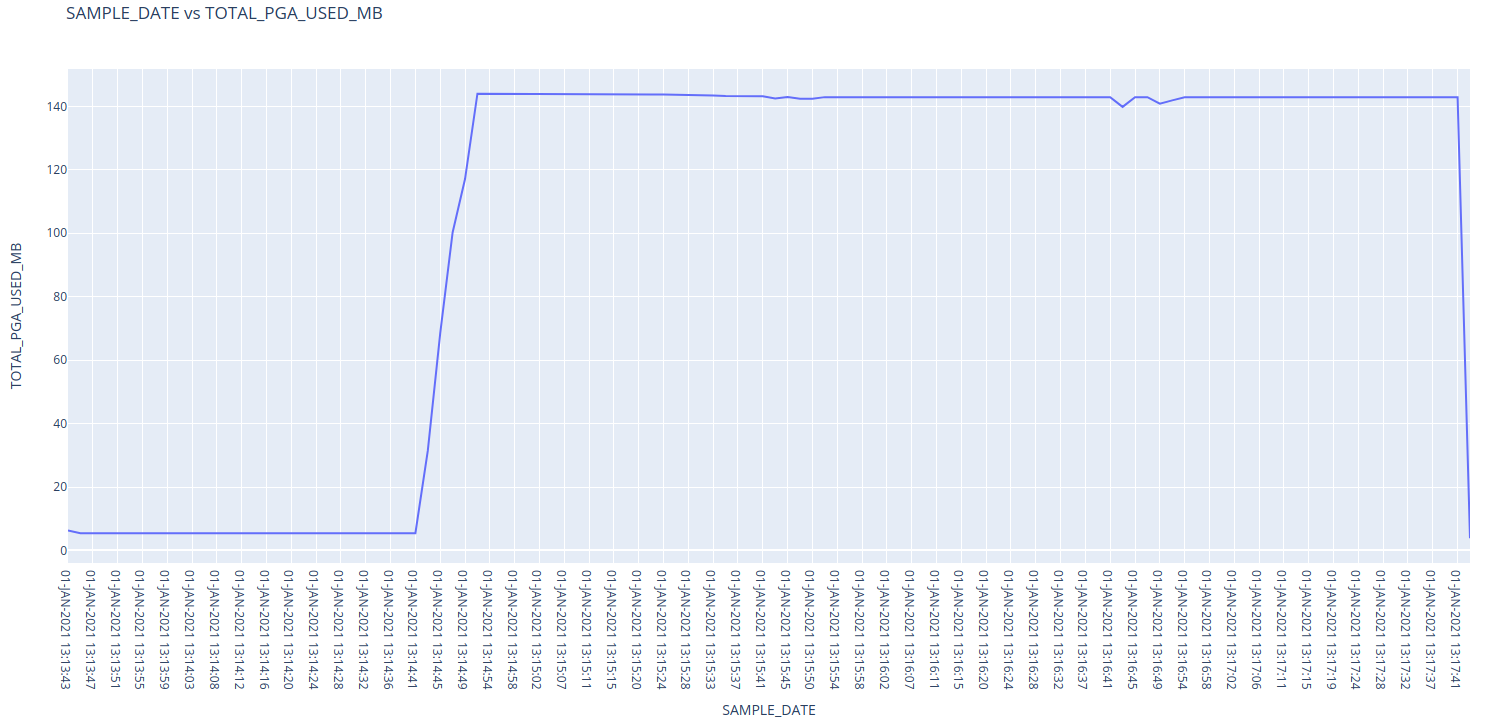
\includegraphics[width=0.9\linewidth]{t06-grafica02-other}
    \caption{Usando \texttt{other-processs}}
  \end{subfigure} 
\end{figure}

Ahora bien, para el caso de los procesos requeridos para los usuarios que
conectan a la base de datos se observa que: para la gráfica (a) y (c), en (a)
prácticamente no se levantan nuevos procesos de \texttt{background}, sin
embargo, si se requieren de \texttt{otros} procesos para poder atender a los 100
usuarios.

Para las gráficas (b) y (d) se observa que para cada tipo de proceso, ya sea de
\texttt{background} u \texttt{otros}, en ambos casos se incrementa la memoria
usada para la PGA. La cantidad de memoria usada se mantiene constante hasta que
los 100 usuarios terminan su ejecución, posteriormente vuelve a la normalidad.

\section*{C6. Salida del validador.}

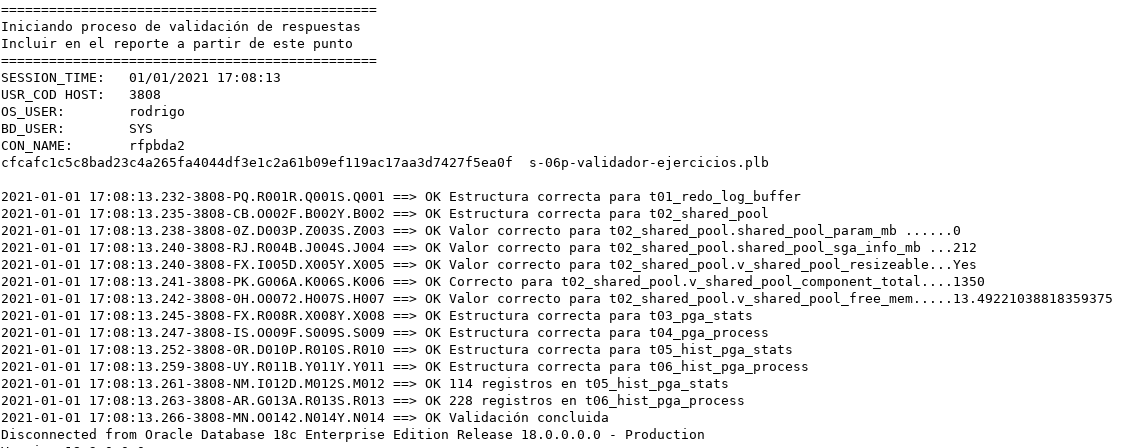
\includegraphics[width=\linewidth]{bda-t04-ep03-validador}

\section*{Comentarios y conclusiones}

Explicar las gráficas me hizo comprender el tema de la administración de las
estructuras de memoria para la PGA y al mismo tiempo comprendi temas posteriores
como la administración de procesos y los tipos de conexión a la base de datos
(dedicado y compartido).

Se comprobó la importancia de las sentencias preparadas para no utilizar más
memoria de la PGA de la cuenta y también se comprendió que existen varios
parámetros de la PGA, algunos nos permiten ver la cantidad de memoria utilizada
mientras que otros nos permiten ver la memoria que se reserva por si el usuario
lanza consultas que puedan requerir más. 

\begin{thebibliography}{99}
    \bibitem{burleson} Burleson Consulting. \textit{Oracle tips } en 
    \texttt{http://www.dba-oracle.com/oracle\_news/}
  \bibitem{oracle} Oracle Help Center. \textit{Database Performance Tuning 
    Guide} en \texttt{https://docs.oracle.com/database/\\%
    121/TGDBA/tune\_buffer\_cache.htm\#TGDBA294}
  \bibitem{campos} Rodriguez Campos, Jorge Alberto. \textit{Administración de
    las estructuras de memoria}. Apuntes de base de datos avanzadas. UNAM
\end{thebibliography}

\end{document}
